% !TEX root = ./busty_transcription.tex
\section{Bayesian inference}
\label{sec:bayesian}

\subsection{The problem of parameter inference}

\mmnote{Bayes theorem. Elaborate on posterior as plausibility over space of
model parameters.} 

One could argue that the whole goal of formulating theoretical models about
nature is to sharpen our understanding from qualitative statements to precise
quantitative assertions about the relevant features of the natural phenomena in
question \cite{Gunawardena2014}. It is in these models that we intend to distill
the essential parts of the object of study. Writing down such models leads to a
propagation of mathematical variables that parametrize our models. By assigning
numerical values to these parameters we can compute concrete predictions that
can be contrasted with experimental data. But for these predictions to match the
data the parameter values have to carefully be chosen from the whole parameter
space. But how do we go about asserting the effectiveness of different regions
of parameter space to speak to the ability of our model to reproduce the
experimental observations? The language of probability, and more specifically of
Bayesian statistics is -- we think -- the natural language to tackle this
question.

\subsubsection{Bayes theorem}

Bayes theorem is a simple mathematical statement that can apply to \textit{any}
logical conjecture. For two particular events $A$ and $B$ that potentially 
depend on each other Bayes theorem gives us a recipe for how to update our 
beliefs about one, let's say $B$, given that we get to observe something about
$A$. In its most classic form Bayes theorem is written as
\begin{equation}
P(B \mid A) = {P(A \mid B) P(B) \over P(A)},
\end{equation}
where the vertical line $\mid$ is read as ``given that''. So $P(B \mid A)$ is
read as probability of $B$ given that $A$ took place. $A$ and $B$ can be any
logical assertion. In particular the problem of Bayesian inference focuses on
the question of finding the probability distribution of a particular parameter
value given the data.

For a given model with a set of parameters $\vec{\theta} = (\theta_1, \theta_2,
\ldots, \theta_n)$, the so-called \textit{posterior distribution} 
$P(\vec{\theta} \mid D)$, where $D$ is the experimental data, quantifies the
plausibility of a set of parameter values given that we get to observe some
particular dataset. In other words, through the application of Bayes formula we
update our beliefs on the possible values that parameters can take upon learning
the outcome of a particular experiment. We specify the word ``update'' as we
come to every inference problem with prior information about the plausibility of
particular regions of parameter space even before performing any experiment.
Even when we claim as researchers that we are totally ignorant about the values
that the parameters in our models can take, we always come to a problem with
domain expertise that can be exploited. If this was not the case, it is likely
that the formulation of our model is not going to capture the phenomena we claim
to want to understand. This prior information is caputerd in the \textit{prior
probability} $P(\vec{\theta})$. The relationship between how parameter values
can connect with the data is enconded in the \textit{likelihood function} $P(D
\mid \vec{\theta})$. Our theoretical model, whether deterministic or
probabilistic, is encoded in this term that can be intuitively understood as the
probability of having observed the particular experimental data we have at hand
given that our model is parametrized with the concrete values $\vec{\theta}$. 
Implicitly here we are also conditioning on the fact that our theoretical model
is ``true,'' i.e. the model itself if evaluated or simulated in the computer is
capable of generating equivalent datasets to the one we got to observe in an 
experiment. In this way Bayesian inference consists of applying Bayes formula 
as 
\begin{equation}
P(\vec{\theta} \mid D) \propto P(D \mid \vec{\theta}) P(\vec{\theta}).
\end{equation}
Notice than rather than writing the full form of Bayes theorem, we limit 
ourselves to the terms that depend on our quantity of interest -- that is the 
parameter values themselves $\vec{\theta}$ -- as the denominator $P(D)$ only
serves as a normalization constant.

\subsubsection{The likelihood function}

\mmnote{Choosing likelihoods. Easy here, just the steady-state distributions of
our master equations, assuming iid single-cell measurements.}

As we alluded in the previous section it is through the likelihood function 
$P(D \mid \vec{\theta})$ that we encode the connection between our parameter 
values and the experimental observables. Broadly speaking there are two classes
of models that we might need to encode into our likelihood function:
\begin{itemize}
        \item Deterministic models: Models for which a concrete selection of
        parameter values give a single output. Say differently, rigid models 
        with a one-to-one mapping between inputs and outputs.
        \item Probabilistic models: As the name says it, models that rather than
        having a one-to-one mapping, describe the full probability distribution
        of possible outputs.
\end{itemize}
In this paper we focus on inference done with probabilistic models. After all
the chemical master equations we wrote down describe the time evolutions of the
mRNA probability distribution. So all our terms $P(\vec{\theta} \mid D)$ will be
given by the steady-state solution of the corresponding chemical master equation
in question. This is rather convenient as we do not have to worry about adding a
statistical model on top of our model to describe deviations from the
predictions; our models themselves focus on predicting such variations from cell
count to cell count.

\subsubsection{Prior selection}

\mmnote{Choosing priors. Not critical here because we are data-rich and
nonhierarchical, as long as we don't exclude ground truth. In other
applications, prior can matter a lot. This is a feature, not a bug: it's
revealing hidden structure that was implied by your modeling assumptions and you
just didn't realize it. Predictive checks to verify you're not excluding any
plausible values.}

The different models explored in this work embraced different levels of
coarse-graining that resulted in a diverse number of parameters for different
models. For each of these model configurations Bayes theorem demands from us to
represent our preconceptions on the possible parameter values in the form of the
prior $P(\vec{\theta})$. Throughout this work for models with $> 1$ parameter we
assign independent priors to each of the parameters; this is
\begin{equation}
P(\vec{\theta}) = \prod_{i=1}^n P(\theta_i).
\end{equation}
Although it is common practice to use non-informative, or maximally
uninformative priors, we are of the mindset that this is a disservice to the
philosophical and practical implications of Bayes theorem. It sounds almost
contradictory to claim that can we represent our thinking about a natural
phenomena in the form of a mathematical model -- which itself is a bold claim of
deeply understanding the features that matter in the object of study -- but we
have absolutely no idea what the parameter values ought to be. We therefore make
use of our own expertise, many times in the form of order-of-magnitude
estimates, to write down prior distributions for our parameters. In summary then
we don’t want to be maximally uninformative because we aren’t completely
uninformed.

For our particular case all of the datasets from~\cite{Jones2014} used in this
paper have $\mathcal{O}(10^3)$ data points. What this implies is that our
particular choice of priors will not significantly affect our inference as long
as they are broad enough. A way to see why this is the case is to simply look at
Bayes theorem. For $N ~ 1000-3000$ datum all of the independent of each other
and $n \ll 10^3$ parameters Bayes theorem reads as
\begin{equation}
P(\vec{\theta} \mid D) \propto \prod_{k=1}^{N} P(d_k \mid \vec{\theta})
\prod_{i=1}^n P(\theta_i),
\end{equation}
where $d_k$ represents the $k$-th datum. That means that if our priors span a
wide range of parameter space, the posterior distribution would be dominated by
the likelihood function.

\mmnote{
\begin{itemize}
% \item Bayes theorem.
% Elaborate on posterior as plausibility over
% space of model parameters.
% \item Choosing likelihoods.
% Easy here, just the steady-state distributions of our master
% equations, assuming iid single-cell measurements.
% \item Choosing priors.
% Not critical here because we are data-rich and nonhierarchical,
% as long as we don't exclude ground truth. In other applications,
% prior can matter a lot. This is a feature, not a bug: it's
% revealing hidden structure that was implied by your modeling
% assumptions and you just didn't realize it. Predictive checks to
% verify you're not excluding any plausible values.
\item Marginalization/expectations.
Analytically hard, trivial with sampling.
\item MCMC.
Lot's of fun here, and deep analogies to stat mech and
Hamiltonian mechanics worth exploring. In a perfect world, you'd
wave a magic wand and generate independent draws from target
posterior. But we don't know how. Next best: generate a Markov
chain of $N$ \textit{correlated} samples, estimate an
autocorrelation time $\tau$, then you've got roughly $N/\tau$
effective samples. Obviously with some assumptions.
\item Posterior predictive checks.
So the posterior is fine, but is the model actually not wrong?
PPC is essential to verify that your model is a plausible
generative process for the data.
\item Discuss identifiability, degeneracy, and failed PPCs in main text. Better thru example anyway.
\end{itemize}
}

\subsection{Bayesian inference on constitutive promoters}
\label{sec:si_bayes_unreg}

Having introduced the ideas behind Bayesian inference we are ready to apply the
theoretical machinery to our non-equilibrium models. In particular in this
section we will focus on model 1 and model 5 in
Figure~\ref{fig2:constit_cartoons}(A). Model 1, the Poisson promoter, will help
us build practical intuition into the implementation of the Bayesian inference
pipeline as we noted in Section~\ref{sec:beyond_means} of the main text that
this model cannot be reconciled with experimental data from observables such as
the Fano factor. In other words, we acknowledge that this model is ``wrong,''
but we still see value in going through the analysis since the simple nature of
the model translates into a neat statistical analysis.

\subsubsection{Model 1 - Poisson promoter}

As specified in the main test, the mRNA steady-state distribution for model 1 in
Figure~\ref{fig2:constit_cartoons}(A) is Poisson with parameter $\lambda$.
Throughout this Appendix we will appeal to the convenient notation for
probability distributions of the form
\begin{equation}
m \sim \text{Poisson}(\lambda),
\end{equation}
where the simbol ``$\sim$'' can be read as \textit{is distributed according to}.
So the previous equation can be read as: the mRNA copy number $m$ is distributed
according to a Poisson distribution with parameter $\lambda$. Our objective then
is to compute the posterior probability distribution $P(\lambda \mid D)$, where,
as in the main text, $D = \{ m_1, m_2, \ldots, m_N \}$ are the data consisting
of single-cell mRNA counts. Since we can assume that each of the cells mRNA
counts are independent of any other cells, our likelihood function $P(D \mid
\lambda)$ consists of the product of $N$ Poisson distributions.

To proceed with the inference problem we need to specify a prior. In this case
we are extremely data-rich, as the dataset from Jones et.\ al~\cite{Jones2014}
has of order 1000-3000 single-cell measurements for each promoter, so our choice
of prior matters little here, as long as it is sufficiently broad. A convenient
choice for our problem is to use a \textit{conjugate} prior. A conjugate prior
is a special prior that causes the posterior to have the same functional form as
the prior, simply with updated model parameters. This makes calculations
analytically tractable and also offers a nice interpretation of the inference
procedure as updating our knowledge about the model parameters. This makes
conjugate priors very useful when they exist. The caveat is that conjugate
priors only exist for a very limited number of likelihoods, mostly with only one
or two model parameters, so in almost all other Bayesian inference problems, we
must tackle the posterior numerically.

But, for the problem at hand, a conjugate prior does in fact exist. For a
Poisson likelihood of identical and identically distributed data, the conjugate
prior is a gamma distribution, as can be looked up in, e.g.,~\cite{Gelman2013},
Section 2.6. Putting a gamma prior on $\lambda$ introduces two new parameters
$\alpha$ and $\beta$ which parametrize the gamma distribution itself, which we
use to encode the range of $\lambda$ values we view as reasonable. Recall
$\lambda$ is the mean steady-state mRNA count per cell, which \textit{a priori}
could plausibly be anywhere from 0 to a few hundred. $\alpha=1$ and $\beta=1/50$
achieve this, since the gamma distribution is strictly positive with mean
$\alpha/\beta$ and standard deviation $\sqrt{\alpha}/\beta$. To be explicit,
then, our prior is
\begin{equation}
\lambda \sim \text{Gamma}(\alpha, \beta)
\end{equation}

As an aside, note that if we did not know that our prior was a conjugate prior,
we could still write down our posterior distribution from its definition as
\begin{equation}
p(\lambda\mid D,\alpha,\beta)
\propto p(D\mid\lambda) p(\lambda \mid\alpha,\beta)
\propto \left(\prod_{k=1}^N \frac{\lambda^{m_k}e^{-\lambda}}{m_k!}\right)
        \frac{\beta}{\Gamma(\alpha)}(\beta\lambda)^{\alpha-1} e^{-\beta\lambda}
.
\end{equation}
Without foreknowledge that this in fact reduces to a gamma distribution, this
expression might appear rather inscrutable. When conjugate priors are
unavailable for the likelihood of interest - which is almost always the case for
models with $>1$ model parameter - this inscrutability is the norm, and making
sense of posteriors analytically is almost always impossible. Fortunately, MCMC
sampling provides us a powerful method of constructing posteriors numerically
which we will make use of extensively.

Since we did use a conjugate prior, we may simply look up our posterior in any
standard reference such as~\cite{Gelman2013}, Section 2.6,
from which we find that
\begin{equation}
\lambda
\sim \text{Gamma}\left(\alpha + \bar{m}N, \beta + N\right),
\end{equation}
where we defined the sample mean $\bar{m} = \frac{1}{N}\sum_k m_k$ for
notational convenience. A glance at the FISH data from~\cite{Jones2014} reveals
that $N$ is $\mathcal{O}(10^3)$ and $\langle m\rangle \gtrsim 0.1$ for all
constitutive strains in~\cite{Jones2014}, so $\bar{m}N \gtrsim 10^2$. Therefore
as we suspected, our prior parameters are completely overwhelmed by the data.
The prior behaves, in a sense, like $\beta$ extra ``data points''
with a mean value of $(\alpha-1)/\beta$~\cite{Gelman2013}, which
gives us some intuition for how much data is needed to overwhelm
the prior in this case: enough data $N$ such that $\beta\ll N$
and $\alpha/\beta \ll \bar{m}$. In
fact, $\bar{m}N$ and $N$ are so large that we can, to an excellent
approximation, ignore the $\alpha$ and $\beta$ dependence and approximate the
gamma distribution as a Gaussian with mean $\bar{m}$ and standard deviation
$\sqrt{\bar{m}/N}$, giving
\begin{equation}
\lambda
\sim \text{Gamma}\left(\alpha + \bar{m}N, \beta + N\right)
\approx \text{Normal}\left(\bar{m}, \sqrt{\frac{\bar{m}}{N}}\right).
\end{equation}
As an example with real numbers, for the \textit{lacUV5} promoter, Jones et.\
al~\cite{Jones2014} measured 2648 cells with an average mRNA count per cell of
$\bar{m} \approx 18.7$. In this case then, our posterior is
\begin{equation}
\lambda
\sim \text{Normal}\left(18.7, 0.08\right),
\label{eq:gauss_posterior}
\end{equation}
which suggests we have inferred our model's one parameter to a precision of
order 1\%.

This is not wrong, but it is not the full story. The model's posterior
distribution is tightly constrained, but is it a good generative model? In other
words, if we use the model to generate synthetic data in the computer does it
generate data that look similar to our actual data, and is it therefore
plausible that the model captures the important features of the data generating
process? This intuitive notion can be codified with \textit{posterior predictive
checks}, or PPCs, and we will see that this simple Poisson model fails badly.

The intuitive idea of posterior predictive checks is simple: 
\begin{enumerate}
\item Make a random draw of the model parameter $\lambda$ from the posterior
distribution.
\item Plug that draw into the likelihood and generate a synthetic dataset
$\{m_k\}$ conditioned on $\lambda$.
\item Repeat many times.
\end{enumerate}
More formally, the posterior predictive distribution can be thought of as the
distribution of future yet-to-be-observed data, conditioned on the data we have
already observed. Clearly if those data appear quite different, the model has a
problem. Put another way, if we suppose the generative model is true, i.e. we
claim that our model explains the process through which our observed
experimental data was generated, then the synthetic datasets we generate should
resemble the actual observed data. If this is not the case, it suggests the
model is missing important features. All the data we consider in this work are
1D (distributions of mRNA counts over a population) so empirical cumulative
distribution functions ECDFs are an excellent visual means of comparing
synthetic and observed datasets. In general for higher dimensional datasets,
much of the challenge is in merely designing good visualizations that can
actually show if synthetic and observed data are similar or not.

For our example Poisson promoter model then, we merely draw many random numbers,
say 1000, from the Gaussian posterior in Eq.~\ref{eq:gauss_posterior}. For each
one of those draws, we generate a dataset from the likelihood, i.e., we draw
2648 (the number of observed cells in the actual dataset) Poisson-distributed
numbers for each of the 1000 posterior draws, for a total of 2648000 samples
from the posterior predictive distribution.

To compare so many samples with the actual observed data, one excellent
visualization for 1D data is ECDFs of the quantiles, as shown for our Poisson
model in~\fig{fig:constit_post_full}(B) in the main text. 

\subsubsection{Model 5 - Bursty promoter}

Let us now consider the problem of parameter inference from FISH data for model
five from~\fig{fig1:means_cartoons}(C). As derived in
Appendix~\ref{sec:gen_fcn_appdx}, the steady-state mRNA distribution in this
model is a negative binomial distribution, given by
\begin{equation}
p(m) = \frac{\Gamma(m+k_i)}{\Gamma(m+1)\Gamma(k_i)}
        \left(\frac{1}{1+b}\right)^{k_i}
        \left(\frac{b}{1+b}\right)^m,
\label{eq:si_neg_bionom}
\end{equation}
where $b$ is the mean burst size and $k_i$ is the burst rate nondimensionalized
by the mRNA degradation rate $\gamma$. As sketched earlier, we can intuitively
think about this distribution through a simple story. The story of this
distribution is that the promoter undergoes geometrically-distributed bursts of
mRNA, where the arrival of bursts is a Poisson process with rate $k_i$ and the
mean size of a burst is $b$.

As for the Poisson promoter model, this expression for the steady-state mRNA
distribution is exactly the likelihood we want to use in Bayes theorem. Again
denoting the single-cell mRNA count data as $D=\{m_1, m_2,\dots, m_N\}$, here
Bayes theorem takes the form
\begin{equation}
p(k_i, b \mid D) \propto p(D\mid k_i,b)p(k_i, b),
\end{equation}
where the likelihood $p(D\mid k_i,b)$ is given by the product of $N$ negative
binomials as in Eq.~\ref{eq:si_neg_bionom}. We only need to choose priors on
$k_i$ and $b$. For the datasets from~\cite{Jones2014} that we are analyzing, as
for the Poisson promoter model above we are still data-rich so the prior's
influence remains weak, but not nearly as weak because the dimensionality of our
model has increased from one to two.

We follow the guidance of~\cite{Gelman2013}, Section 2.9 in opting for
weakly-informative priors on $k_i$ and $b$ (conjugate priors do not exist for
this problem), and we find ``street-fighting estimates''~\cite{Mahajan2010} to
be an ideal way of constructing such priors. The idea of weakly informative
priors is to allow all remotely plausible values of model parameters while
excluding the completely absurd or unphysical.

Consider $k_i$. Some of the strongest known bacterial promoters control rRNA
genes and initiate transcripts no faster than $\sim 1/\text{sec}$. It would be
exceedingly strange if any of the constitutive promoters from~\cite{Jones2014}
were stronger than that, so we can take that as an upper bound. For a lower
bound, if transcripts are produced too rarely, there would be nothing to see
with FISH. The datasets for each strain contain of order $10^3$ cells, and if
the $\langle m \rangle = k_i b/\gamma \lesssim 10^{-2}$, then the total number
of expected mRNA detections would be single-digits or less and we would have
essentially no data on which to carry out inference. So assuming $b$ is not too
different from 1, justified next, and an mRNA lifetime of $\gamma^{-1}\sim
3-5~\text{min}$, this gives us soft bounds on $k_i/\gamma$ of perhaps $10^{-2}$
and $3\times 10^1$.

Next consider mean burst size $b$. This parametrization of the geometric
distribution allows bursts of size zero (which could representing aborted
transcripts and initiations), but it would be quite strange for the mean burst
size $b$ to be below $\sim10^{-1}$, for which nearly all bursts would be of size
zero or one. For an upper bound, if transcripts are initiating at a rate
somewhat slower than rRNA promoters, then it would probably take a time
comparable to the lifetime of an mRNA to produce a burst larger than 10-20
transcripts, which would invalidate the approximation of the model that the
duration of bursts are instantaneous compared to other timescales in the
problem. So we will take soft bounds of $10^{-1}$ and $10^1$ for $b$.

Note that the natural scale for these ``street-fighting estimates'' was a log
scale. This is commonly the case that our prior sense of reasonable and
unreasonable parameters is set on a log scale. A natural way to enforce these
soft bounds is therefore to use a lognormal prior distribution, with the soft
bounds set $\pm2$ standard deviations from the mean.

With this, we are ready to write our full generative model as
\begin{equation}
\begin{split}
\ln k_i \sim \text{Normal}(-0.5, 2),
\\
\ln b \sim \text{Normal}(0.5, 1),
\\
m \sim \text{NBinom}(k_i, b).
\end{split}
\end{equation}
Section~\ref{section_04_bayesian_inference} in the main text details the
results of applying this inference to the single-cell mRNA counts data.

\subsection{Bayesian inference on the simple-repression architecture}

As detailed in~\ref{section_04_bayesian_inference} in the main text the
inference on the unregulated promoter served as a stepping stone towards our
ultimate goal of inferring repressor rates from the steady-state mRNA
distributions of simple-repression architectures. For this we expand the
one-state bursty promoter model to a two-state promoter as schematized in
Figure~\ref{fig1:means_cartoons}(C) as model 5. This model adds two new
parameters: the repressor binding rate $k^+$, solely function of the repressor
concentration, and the repressor dissociation rate $k^-$, solely a function of
the repressor-DNA binding affinity.

The structure of the data in~\cite{Jones2014} for regulated promoters tuned
these two parameters independently. In their work the production of the LacI
repressor was under the control of an inducible promoter regulated by the TetR
repressor as schematized in Figre~\ref{figS:aTc_circuit}. When TetR binds to the
small molecule anhydrotetracycline (aTc), it shifts to an inactive conformation
unable to bind to the DNA. This translates into an increase in gene expression
level. In other words, the higher the concentration of aTc added to the media,
the less TetR repressors that can control the expression of the \textit{lacI}
gene, so the higher the concentration of LacI repressors in the cell.

\begin{figure}[h!]
\centering
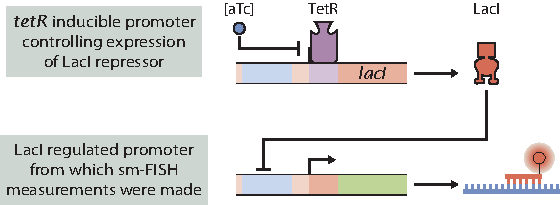
\includegraphics{../figures/si/figS0X_aTc_circuit.pdf}
\caption{\textbf{aTc controlled expression of LacI repressor.} Schematic of the
circuit used in~\cite{Jones2014} to control the expression of the LacI
repressor. The \textit{lacI} gene is under the control of the TetR repressor. As
the TetR repressor is inactivated upon binding of anhydrotetracycline or aTc,
the more aTc added to the media were cells are growing, the less TetR repressors
available to control the expression of the \textit{lacI} gene, resulting in more
LacI repressors per cell. LacI simultaneously controls the expression of the
mRNA on which single-molecule mRNA FISH was performed for gene expression
quantification.}
\label{figS:aTc_circuit}
\end{figure}

As we found in Section~\ref{sec:beyond_means}, for our purposes
the ``right'' model of a constitutive promoter is the bursty
picture, model five in Figure~\ref{fig:constit_cartoons}.
Therefore our starting point here is the analogous model with
repressor added, model 5 in Figure~\ref{fig1:means_cartoons}.
For a given repressor binding site and copy number,
this model has four rate parameters to be inferred:
the repressor binding and unbinding rates $k_R^+$, and $k_R^-$,
the initiation rate of bursts, $k_i$, and the mean burst size $b$
(we nondimensionalize all of these by the mRNA degradation rate $\gamma$).

Before showing the mathematical formulation of our statistical
inference model, we would like to sketch the intuitive structure.
The dataset from~\cite{Jones2014} we consider consists of
single-cell mRNA FISH measurements of nine different conditions,
spanning several combinations of three unique binding sites and
four unique repressor copy numbers. We assume that the values of
$k_i$ and $b$ are known, since we have already cleanly inferred
them from constitutive promoter data, and further we assume that
these values are the same across datasets with different
repressor binding sites and copy numbers. We assume that there is
one unbinding rate parameter for each repressor binding site,
which is shared across conditions, and likewise one binding rate
for each unique repressor copy number. This makes our model seven
dimensional, or nine if one counts $k_i$ and $b$ as well.

Formally now, denote the set of seven repressor rates to be inferred as
\begin{equation}
\vect{k} =\{k_{Oid}^-, k_{O1}^-, k_{O2}^-,
k_{0.5}^+, k_{1}^+, k_{2}^+, k_{10}^+\}.
\end{equation}
Note the repressor copy numbers are not known directly, so we label their
association rates by the concentration of a small molecule inducer aTc
which indirectly controls the transcription of $\textit{lacI}$.
Also note that the authors of~\cite{Jones2014} report estimates
of LacI copy number per cell rather than direct measurements.
However, these estimates were made \textit{assuming} the validity
of the equilibrium models in Figure~\ref{fig1:means_cartoons},
and since \textit{testing} these models is our goal, we will make
no assumptions about the LacI copy number for given aTc concentrations.

Bayes theorem reads simply
\begin{equation}
p(\vect{k}, k_i, b \mid D)
\propto
p(D \mid\vect{k}, k_i, b) p(\vect{k}, k_i, b),
\end{equation}
where $D$ is the set of all $N$ observed single-cell mRNA counts
across the various conditions. We assume that individual single-cell
measurements are independent so that the likelihood factorizes as
\begin{equation}
p(D \mid\vect{k}, k_i, b)
= \prod_{j=1}^N p(m\mid \vect{k}, k_i, b)
= \prod_{j=1}^N p(m\mid k_j^+, k_j^-, k_i, b)
\end{equation}
where $k_j^\pm$ represent the appropriate binding and unbinding
rates for the $j$-th measured cell. The probability
$p(m\mid k_j^+, k_j^-, k_i, b)$ appearing in the last expression
is exactly Eq.~\ref{eq:p_m_bursty+rep_appdx}, the steady-state
distribution for our bursty model with repression derived in
Section~\ref{sec:gen_fcn_appdx}, which for completeness we reproduce here as
\begin{equation}
\begin{split}
p(m \mid k_R^+, k_R^-, k_i, b) = & ~\frac{
        \Gamma(\alpha + m)\Gamma(\beta + m)\Gamma(k_R^+ + k_R^-)
        }
        {
        \Gamma(\alpha)\Gamma(\beta)\Gamma(k_R^+ + k_R^- + m)
        }
\frac{b^m}{m!}
\\
&\times {_2F_1}(\alpha+m, \beta+m, k_R^++k_R^-+m; -b).
\end{split}
\label{eq:p_m_bursty+rep}
\end{equation}
where $\alpha$ and $\beta$, defined for notational convenience, are
\begin{align}
\begin{split}
\alpha &= \frac{1}{2}
\left(k_i+k_R^-+k_R^+ + \sqrt{(k_i+k_R^-+k_R^+)^2 - 4k_i k_R^-}\right)
\\
\beta &= \frac{1}{2}
\left(k_i+k_R^-+k_R^+ - \sqrt{(k_i+k_R^-+k_R^+)^2 - 4k_i k_R^-}\right).
\end{split}
\end{align}

\mmnote{Probably SI most of this paragraph?}
This likelihood is rather inscrutable. We did not find any of the
known analytical approximations for ${_2F_1}$ terribly useful in
gaining intuition, so we instead resorted to numerics. One insight we found
\mmnote{a plot would probably help explain, maybe SI, need to explain better}
was that for very strong or very weak repression, the distribution in
Eq.~\ref{eq:p_m_bursty+rep} is well approximated by a negative binomial
with burst size $b$ and burst rate $k_i$ equal to their
constitutive \textit{lacUV5} values, except with $k_i$ multiplied
by the fold-change $\left(1+k_R^+/k_R^-\right)^{-1}$.
In other words, once again only the \textit{ratio} $k_R^+/k_R^-$
was detectable. But for intermediate repression, the distribution
was visibly broadened with Fano factor greater than $1+b$, the
value for the corresponding constitutive case. This indicates
that the repressor rates had left an imprint on the distribution,
and perhaps intuitively, this intermediate regime occurs for values of
$k_R^\pm$ comparable to the burst rate $k_i$. Put another way,
if the repressor rates are much faster or much slower than $k_i$,
then there is a timescale separation and effectively only one
timescale remains, $k_i\left(1+k_R^+/k_R^-\right)^{-1}$.
Only when all three rates in the problem are comparable does the
mRNA distribution retain detectable information about them.

Next we specify priors. As for the constitutive model, weakly
informative lognormal priors are a natural choice for all our
rates. We found that if the priors were too weak, our MCMC
sampler would often become stuck in regions of parameter space
with very low probability density, unable to move. We struck a
balance in choosing our prior widths between helping the sampler
run while simultaneously verifying that the marginal posteriors
for each parameter were not artificially constrained or distorted
by the presence of the prior. The only exception to this is the
highly informative priors we placed on $k_i$ and $b$, since we
have strong knowledge of them from our inference of constitutive
promoters above.

With priors and likelihood specified we may write down our complete generative model as
\begin{equation}
\begin{split}
\log_{10}k_i &\sim \text{Normal}(0.725, 0.025)\\
\log_{10}b   &\sim \text{Normal}(0.55, 0.025)\\
\log_{10}k_{0.5}^+ &\sim \text{Normal}(-0.45, 0.3)\\
\log_{10}k_{1}^+   &\sim \text{Normal}(0.6, 0.3)\\
\log_{10}k_{2}^+   &\sim \text{Normal}(1.15, 0.3)\\
\log_{10}k_{10}^+  &\sim \text{Normal}(1.5, 0.3)\\
\log_{10}k_{Oid}^- &\sim \text{Normal}(-0.25, 0.3)\\
\log_{10}k_{O1}^-  &\sim \text{Normal}(0.1, 0.3)\\
\log_{10}k_{O2}^-  &\sim \text{Normal}(0.45, 0.3)\\
m &\sim \text{Likelihood}(k_R^+, k_R^-, k_i, b),
\end{split}
\end{equation}
where the likelihood is specified by Eq.~\ref{eq:p_m_bursty+rep}.
\mmnote{Now that I've typed this out, this notation seems totally
pointless here, especially when the likelihood is not a standard
distribution. Maybe I should make a table or something to record
the prior values, and maybe even that should go to SI?}
We ran MCMC sampling on the full nine dimensional posterior
specified by this generative model. To attempt to visualize this
object, in Figure~\ref{fig4:repressed_post_full}(A) we plot
several two-dimensional slices as contour plots, analogous to
Figure~\ref{fig:constit_post_full}(C). Each of these nine slices
corresponds to the $(k_R^+, k_R^-)$ pair of rates for one of the
conditions from the dataset used to fit the model and gives a
sense of the uncertainty and correlations in the posterior.

\mmnote{Outline:
\begin{itemize}
\item Hey look it mostly works. With full model, 9D model is well identified,
though most of the individual experiments unsurprisingly are not:
only 3 of the 9 datasets were identifiable if fit in isolation
and for the rest only the ratio of repressor rates is identifiable.
Only by making assumptions that certain rates
are equal across datasets was identifiability achieved.
PPC is not perfect, it kinda misses some
rep/op pairs but overall it's surprisingly predictive considering how strong
were the assumptions that went into it.
\item Do we chalk this up to experimental imperfections or is there interesting
biology to be found in the disagreements? I'm inclined towards the former. Even
just catching cells in truly apples-to-apples growth phases, or matching up
parameters of imaging sessions weeks or months apart, is hardly trivial.
\item The alternative is to refine our model and/or add on complexity, and it's
not at all clear what additions to make to the model, especially how to produce
the long tail of repressed strains over UV5. I see no way to get that without
getting into complicated time-correlation/history effects, where
transcription...rebounds?? After being repressed?? Sounds odd.
\item Comparison between my inferred rates, equilibrium binding E, and
single-molecule measurements. Not quite as slam-dunk as I'd hoped because of
$\gamma$ dependence, but rates are w/in factor of 2 or better, seems quite good
really! With exception of one Oid data data point, free energies are w/in about
0.5 kT also. That's not massively larger than the repeatability threshold of
fold-change measurements, at maybe 0.1 to 0.3 kT.
\item Surprising that so many model parameters can be inferred from just a few
distributions that, by eye, don't have strong features! Does require some
assumptions, e.g., about equivalence of rates across experiments, but that seems
quite reasonable.
\end{itemize}
}

\mmnote{These next 2 paragraphs should be SI, I think. Leaving here for
now to avoid a merge conflict w/ MRM.}

We found that fitting a single operator/aTc concentration at a
time with a single binding and unbinding rate did not yield a
stable inference for most of the possible operator/aTc
combinations. In other words, a single dataset could not
independently resolve the binding and unbinding rates, only their
ratio as set by the mean fold-change in
Figure~\ref{fig1:means_cartoons}. Only by making the assumption
of a single unique binding rate for each repressor copy number
and a single unique unbinding rate for each binding site, as done
in Figure~\ref{fig4:repressed_post_full}A, was it possible to
independently resolve the rates and not merely their ratios.

We also note that we found it necessary to exclude the very
weakly and very strongly repressed datasets from Jones et.\
al.~\cite{Jones2014}. In both cases there was, in a sense, not
enough information in the distriubtions for our inference
algorithm to extract, and their inclusion simply caused problems
for the MCMC sampler without yielding any new insight. For the
strongly repressed data (Oid, 10~ng/mL aTc), with $>$ 95\% of cells
with zero mRNA, there was quite literally very little data from
which to infer rates. And the weakly repressed data, all with the
repressor binding site O3, had an unbinding rate so fast that the
sampler essentially sampled from the prior; the likelihood had
negligible influence, meaning the data was not informing the
sampler in any meaninful way, so no inference was possible.